% Chapter 1: Introduction

\chapter{Introduction}
\label{sec:introduction}

Plasmas are fluid masses of charged particles, often formed when neutral atoms and molecules in a gas are ionized by external energy.  Instances of plasma include everything from florescent lightbulbs and flames to more exotic examples such as nuclear fusion reactor experiments, most stars, nebula, and the interstellar medium.  In fact, about 99\% of matter in the known universe exists in the plasma state.  Of particular interest to this thesis is the plasma in Earth's ionosphere.

Ionospheric plasma is partially ionized, meaning only a fraction of the particles are ionized and the rest are neutral.  Considering the dynamics of plasmas therefore requires not only collisions between particles to be considered but also charge-charge interactions and external and internal electric and magnetic fields.  These dynamics can generate waves in the plasma, which cause density perturbations.  Additionally, variations in temperature and electric and magnetic field strength can occur on a variety of scales.  This thesis focuses on mechanisms by which density variations in ionospheric plasma occur, often referred to as plasma structures.

\section{The Solar-Terrestrial Environment}
The solar terrestrial environment begins with the Sun in the center of the solar system.  The Sun is composed of highly energized plasma that is gravitationally bound together.  The surface of the Sun is highly dynamic, populated with sunspots, which are dark, relatively cool regions with intense magnetic fields, as well as coronal holes, which are low density areas characterized with a continuous outflow of plasma.  The intense magnetic fields associated with sunspots can break down releasing a large amount of energy and plasma, known as a solar flare.  Planet-sized masses of plasma known as coronal mass ejections (CMEs) can be ejected from the surface, which can be large enough to maintain an internal magnetic field as they travel through the solar system.  The frequency of sunspots and large outbursts of plasma changes with the 11-year long solar cycle.  A large number of sunspots, high occurrence of fast, dense plasma outbursts, and a highly variably magnetic field indicate solar maximum.  Conversely, solar minimum is characterized by a low sunspot number and slow and relatively steady outflow.  This thesis examines factors that control irregularity production in the Earth's ionosphere, which can be strongly influenced by solar activity.

The Sun interacts with the rest of the solar system through the solar wind, a continuous outflow of plasma that caries the Sun's magnetic field with it.  This is shown in Figure \ref{fig:ste}.  The solar wind, represented by the green arrows, typically has a density around 10 cm\(^{-3}\) and is traveling away from the Sun at approximately 400 km/s at Earth's orbit.  However, like the Sun, the solar wind is highly dynamic and these parameters can change drastically over a period of minutes.  CMEs, for instance, create a substantial increase in density and are often preceded by a shock, a region of hot, compressed plasma caused by the CME moving at supersonic speeds.  In addition to the outflow of plasma, the solar wind also consists of the Sun's magnetic field extended into the outer limits of the solar system, called the interplanetary magnetic field (IMF), dark blue lines in Figure \ref{fig:ste}.  Because the Sun has a short rotation period (about 33 days), the IMF gets twisted into a spiral, commonly called the Parker Spiral \citep{Parker1958}.  When the IMF reaches the Earth, the magnetic field is typically oriented at a \(45\deg\) inclination relative to the ecliptic, but this is highly variable depending on solar wind conditions.

\begin{figure}
	\includegraphics[width=\textwidth,angle=0]{ste.pdf}
	\caption[Solar-Terrestrial Environment]{Diagram of the solar-terrestrial environment.  The solar wind, green arrows, contains both a steady stream of charged particles and the IMF, dark blue.  The red region represents the magnetosheath.  The manetopause is shown by the black dashed line.  Closed magnetic field lines from the earth are shown in grey while open field lines are shown in light blue.  The ionosphere is shown in light green above the Earth's surface.}
	\label{fig:ste}
\end{figure}

The IMF interacts with the Earth's own magnetic field, and this interaction creates the magnetosphere.  Without the IMF, the magnetosphere would be approximately a dipole field, but dynamic pressure from the solar wind causes the Sun facing side to be compressed to 6--10 Earth radii and the rear side to be stretched into an extended tail (hundreds of Earth radii).  Because the solar wind is typically a supersonic flow, a bow shock forms on the dayside of the magnetosphere.  The heated and compressed solar wind plasma created by the bow shock is known as the magnetosheath, the red region in Figure \ref{fig:ste}.  The magnetopause, black dashed line, is the actual boundary between solar wind plasma in the magnetosheath and magnetospheric plasma.  Magnetic field lines that are part of the closed magnetosphere are shown in grey in Figure \ref{fig:ste}.  However, the magnetosphere is not fully closed.  At the magnetopause, magnetic reconnection can occur between the IMF and the Earth's magnetic field creating open field lines, light blue in Figure \ref{fig:ste}.  This reconnection occurs on last closed field line intersecting the magnetopause (highlighted in yellow in Figure \ref{fig:ste}).  Magnetic field lines originating from the Earth are then directly connected to the Sun through the solar wind, which consequently allows highly energized solar particles to enter the magnetosphere.  Open field lines tend to occur around the Earth's polar caps, making these regions particularly interesting to study due to very complex behavior and coupled interactions between the Earth and the Sun.

Closer to the Earth's surface, the magnetosphere also interacts with the Earth's ionosphere, a layer of partially ionized plasma in the upper atmosphere, light green in Figure \ref{fig:ste}.  The interaction between charged particles in the ionosphere with magnetic field lines couples the ionosphere, magnetosphere, and solar wind to create non-trivial dynamics.  Additionally,  neutral winds in the thermosphere can influence the ionosphere through viscous interactions.  Overall, the charged particle interactions in the ionosphere create a highly complex system, which is further complicated by coupling with both the thermosphere from below and the magnetosphere and solar wind from above.  

\section{The Earth's Ionosphere}
\label{sec:ionosphere}
The Earth's ionosphere is a region of the upper atmosphere that ranges approximately between 50--1000 km in altitude where neutral gases have been partially ionized, resulting in free electrons and ions mixed with neutral particles.  Two competing processes occur in the ionosphere to create a peak in electron density.  Solar illumination and particle precipitation ionize neutrals, and the density of ions increase as altitude decreases because there are more neutral molecules available to ionize.  However, below a certain point, the concentration of ions becomes large enough that recombination into neutral particles becomes a substantial factor, reducing the ion density.  The exact altitude where this density peak occurs is variable with time of day, location, season, and solar cycle.  A profile of how electron density changes with altitude is shown in Figure \ref{fig:densprofile}, found from the International Reference Ionosphere (IRI) model run on January 1, 2007 at \(75\deg\) N, \(0\deg\) E, geographic (the IRI model is discussed further in Section \ref{sec:iri}).

\begin{figure}
	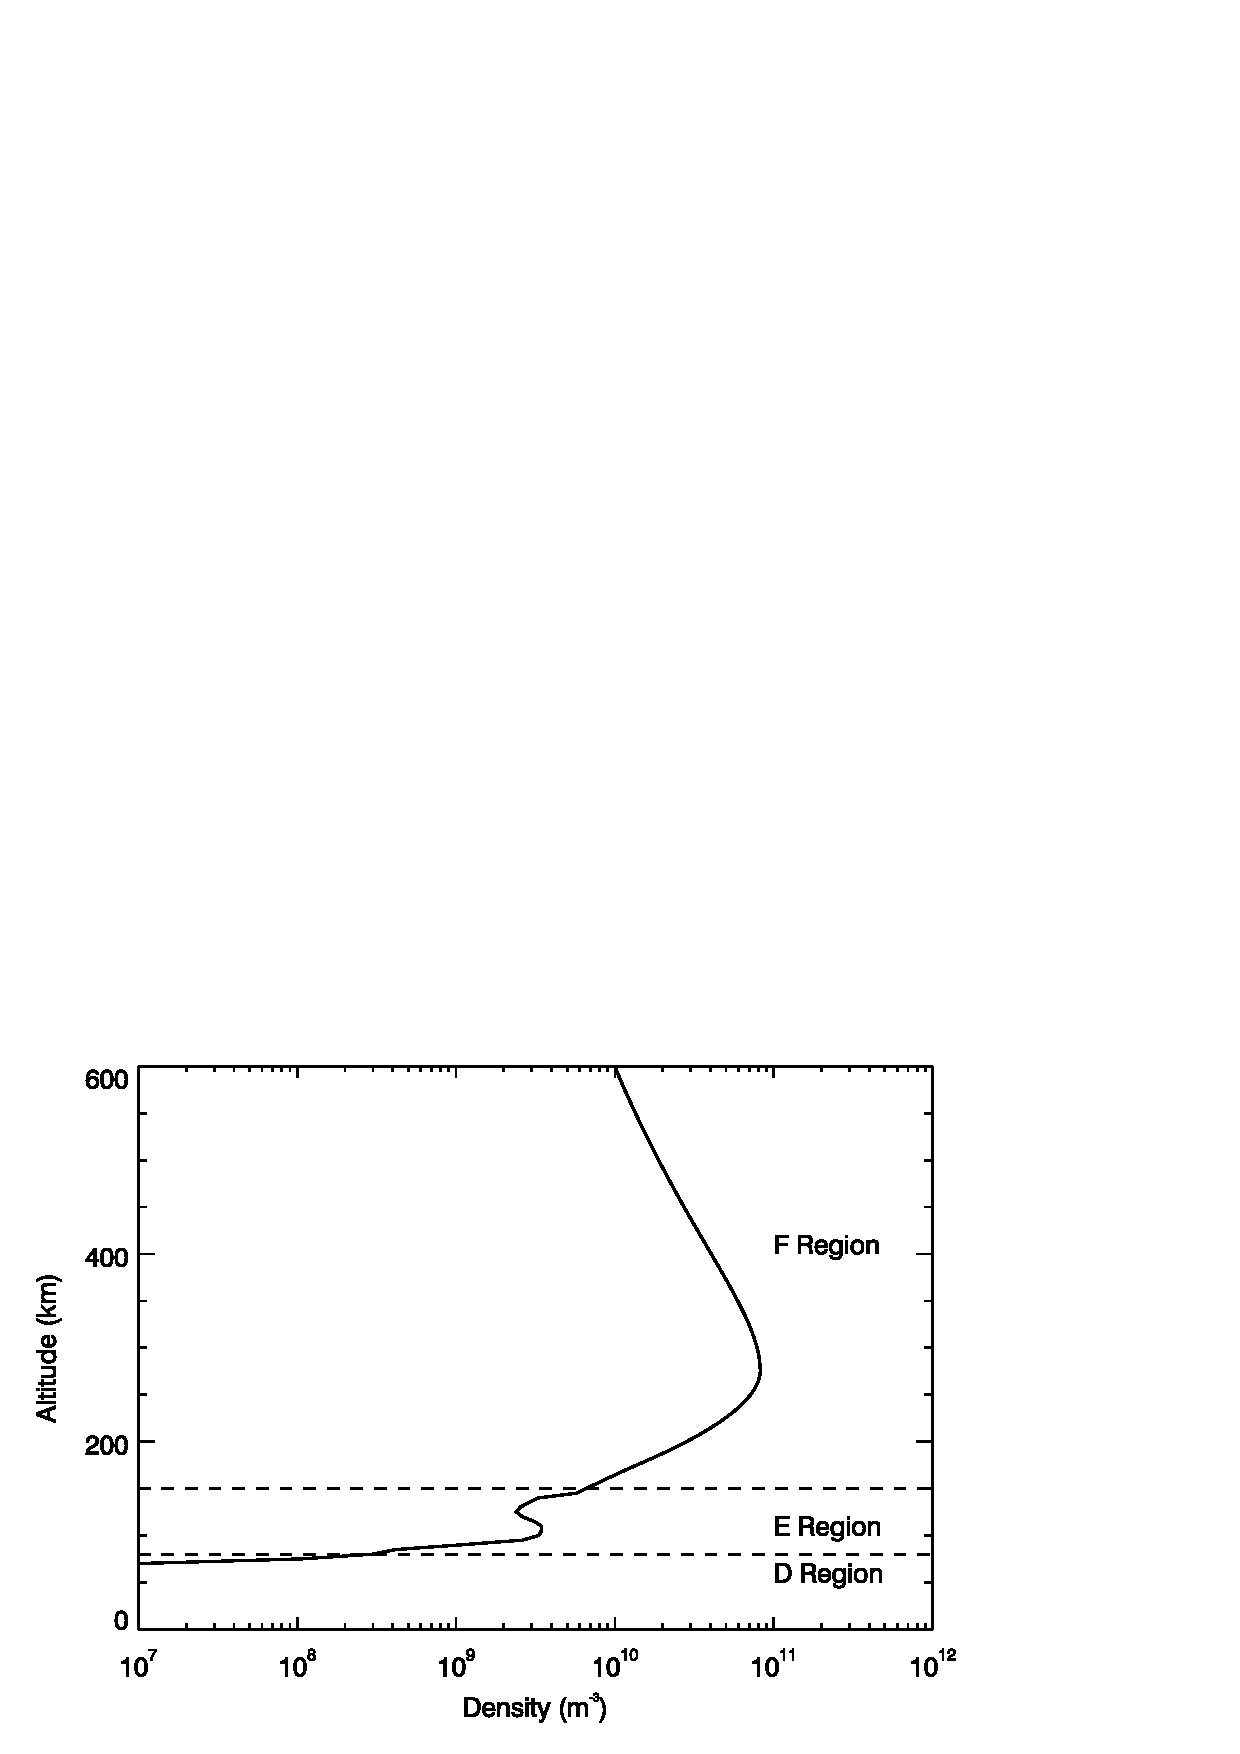
\includegraphics[width=\textwidth]{densprofile.pdf}
	\caption[Ionosphere density profile]{Altitude profile of electron density throughout the ionosphere found from the IRI model.  Typical ranges of the \(D\), \(E\), and \(F\) regions are identified.}
	\label{fig:densprofile}
\end{figure}

Above 50 km, the primary neutral particles are atomic oxygen, O, molecular oxygen, O\(_2\), and molecular nitrogen, N\(_2\).  Common ions at these altitudes are therefore mostly composed of oxygen and nitrogen, O\(^+\), NO\(^+\), O\(_2^+\), N\(_2^+\), but hydrogen, H\(^+\), can contribute as well, particularly at higher altitudes \citep{Kelley2009}.  In the ionosphere, neutral densities are typically several orders of magnitude higher than ion densities, however even a small number of charged particles changes the behavior of the region dramatically.  Because there are so many different ion species, plasma density is usually discussed simply in terms of electron density.  Plasmas are assumed to be quasineutral, meaning that electron and ion densities are approximately the same so the plasma does not have an overall charge.  The electron density is equal to the sum of densities of all the ions in the plasma, or \(n = n_e = \sum n_i\).

\subsection{Ionospheric Regions}
\label{sec:ionosphere_regions}
The ionosphere is typically divided into three regions, Figure \ref{fig:densprofile}.  The D region is located between 80 and 90 km in altitude and typically only exists in the daytime when the ionosphere is sunlit.  The E region typically exists between 90 and 130 km with a density peak between 105 and 110 km, depending on factors such as time of day and season.  Above 130 km is considered to be the F region, which has a density peak around 250 km, Figure \ref{fig:densprofile} \citet{Luhmann1995}.  The F region can actually have two peaks under some daytime conditions, notated as the F1 peak and the F2 peak.  The peak heights and densities of each of these regions is highly variable both diurnally and seasonally.  In Figure \ref{fig:densprofile}, the daytime profile is shown with the solid line next to a nighttime profile with a dashed line.  Note that night electron densities are lower at all altitudes due to the lack of photoionization during nighttimes.  In addition, the F-region peak moves to higher altitudes at night.  The focus of this thesis will be the F region.

Because the concentrations of ions and neutral particles changes with altitude, each of these regions have distinct plasma physical properties that make them unique.  The main issue is whether the the large-scale motion of a particle is controlled more by the magnetic field (the particle is magnetized) or by collisions with other particles (the particle is collisional).  This can be determined by comparing the collision frequency, \(\nu_\alpha\), to the gyrofrequency, \(\Omega_\alpha\), of a particular species, where \(\alpha\) corresponds to either electrons, \(e\), or ions, \(i\).  If \(\Omega_\alpha \gg \nu_\alpha\), the particle completes many gyrations between each collision, so its motion is determined mostly by the magnetic field and it is magnetized.  If \(\nu_\alpha \gg \Omega_\alpha\), the particle collides with other particles much more often than it complete a gyration, so it is considered collisional.  The gyrofrequency is dependent on the mass and charge of the particle and the strength of the magnetic field, \(\Omega_\alpha = q_\alpha B/m_\alpha\), so is roughly constant through the ionosphere because the magnetic field strength does not change much throughout these altitudes.  The collision frequency depends on the density of a species relative to the density of all other species in the plasma and can be calculated from a series of standard expressions \citep{Schunk1980,Schunk2009}.  In the E region, \(\Omega_e \gg \nu_e\), so electrons are magnetized.  However, the motion on ions is dominated by collisions between ions and neutrals (\(\nu_i > \Omega_i\)), so ions in the \(E\) region are considered collisional.  In the \(F\) region where the neutral density is much lower, both ions and electrons are magnetized, \(\Omega_\alpha \gg \nu_\alpha\).  These differences in how charged particles move impact the conductivity and plasma waves development, which is further discussed in Section \ref{sec:lit_theory}.

\subsection{Plasma Structuring in the Polar Ionosphere}
\label{sec:polar_structure}

This thesis is concerned with the polar ionosphere, which is a particularly interesting and dynamic region due to the presence of open field lines to the solar wind.  The main focus of this work will be plasma density perturbations, often called irregularities.  Density irregularities in the polar cap can occur on scales ranging from thousands of kilometers to less than a centimeter \citep{Tsunoda1988}, and a summary of some of these irregularities is presented in Figure \ref{fig:polarirreg}.  

Large-scale plasma irregularities are typically considered to be any density structure on the scale of greater than 30 km \citep{Kelley2009}.  Some common examples are polar patches, polar holes, and sun-aligned arcs.  Polar patches are large density enhancements (usually at least twice the background plasma density) that travel across the polar cap with the background convection, Figure \ref{fig:polarirreg}a \citep{Weber1984,Valladares1994}.  Polar holes are plasma density depletions that typically occur in the \(F\) region slightly poleward of the auroral oval \citep{Benson2001}.  Sun-aligned arcs are large density forms that stretch across the polar cap along the sun-earth line.  They are very narrow and often characterized by large and complex velocity shears on either side of the arc \citep{Valladares1991}.  Large scale plasma structures and the density gradients that surround them often serve as a platform for smaller-scale structures to form as well.  Polar patches, for instance, are known to form large finger-like structures along their trailing edges, Figure \ref{fig:polarirreg}b \citep{Gondarenko2004b,Hosokawa2016}.

\begin{figure}
	\includegraphics[width=0.5\textwidth]{irregularity.pdf}
	\caption[Plasma irregularities in the polar ionosphere]{Plasma density irregularities occur in the polar cap at different scale sizes.  Polar patches, orange, move with the background ionospheric convection, indicated by red contours (a).  Smaller-scale structures often move develop along the edges of polar patches where strong density gradients exist (b).  Intermediate scale irregularities are primarily responsible for disrupting radio signals traveling through the ionosphere (c).  Field-aligned irregularities, FAIs, are density perturbations that form along the magnetic field lines, light blue (d).}
	\label{fig:polarirreg}
\end{figure}

Intermediate-scale plasma irregularities are those ranges from 100 m -- 30 km \citep{Kelley2009}.  These are also referred to as scintillation-causing structures and are responsible for many of the negative space weather effects that are observed on Earth.  One important example of a space weather effect is when the ionosphere changes the phase and amplitude of the original signal, called radio scintillation, which affects the ability of satellites to communicate with ground receivers.  This can cause communication blackouts or introduce large errors into GPS/GNSS (Global Positioning System/Global Navigation Satellite System) calculations, affecting navigation.

Small-scale structuring is generally considered to be all irregularities less than 100 m \citep{Kelley2009}.  Although small-scale irregularities are not responsible for scintillation that directly impact GPS/GNSS performance, they can be the easiest to study because of large data sets collected from high frequency ionospheric radars globally for several decades (discussed further in Section \ref{sec:superdarn}).  Because electrons move far more easily along magnetic field lines than across them, density perturbations tend to be aligned with the magnetic field and are often known as field-aligned irregularities (FAI), Figure \ref{fig:polarirreg}d.  The irregularity classifications presented here are rough categories only and a high degree of coupling between different scales occurs, which makes plasma structures of all scales (large, intermediate, and small) important for plasma structuring processes.  For instance, large-scale structures such as polar patches may very well have internal intermediate- and/or small-scale structuring.  A turbulent cascade is often assumed to connect these different scales, but because various instruments or techniques usually only observe structuring on a particular scale, it is difficult to find direct evidence of this or how exactly it occurs \citep{Kintner1985,Tsunoda1985}.  A description of some of the particular instruments and models that are used in this thesis follows.

\section{Observational Techniques and Models}

\subsection{Coherent Scatter Radars}
\label{sec:csr}
In this thesis, we make extensive use of Coherent Scatter Radars (CSR), which have been used to study the ionosphere for the last half century.  The radar transmits a radio wave, which can scatter off plasma structures in the ionosphere, and then be detected by the receiving antennas.  The time difference between when the signal was transmitted and when it was detected and the power and phase of the returned signal can then be used to determine characteristics of plasma irregularities.

There are three measurements typically made by CSR systems: backscatter power, line-of-sight (LoS) velocity, and spectral width.  Backscatter power is the power of the returned signal that the radar's receivers detect.  Typically, a threshold is selected for the minimum power acceptable for a return to be considered an actual signal instead of background noise.  LoS velocity is the component of the total plasma drift velocity that is measured along the transmitted signal direction.  Because radars measure velocity through the doppler shift of backscatter, only the component of the velocity vector can be measured.  Spectral width represents the width of the doppler power spectrum and can determine characteristics of irregularities \citep{Greenwald1985}.

CSR systems can operate by transmitting pulses instead of continuously.  This allows the distance between the radar and the target to be found (based on the time difference between when the pulse is transmitted and received).  The size of the range gate is determined by the length of a radar pulse, Equation \ref{eqn:range_gate}.
\begin{equation}
	\label{eqn:range_gate}
	\Delta r = \frac{c\Delta t}{2}
\end{equation}.
Here, \(\Delta r\) is the size of a range gate, \(\Delta t\) is the pulse length, and \(c\) is the speed of light.  Longer pulses result in larger range gates, resulting in poorer spatial resolution.

When the radar transmits continuously, backscatter will be received, but because it is impossible to know when that signal was transmitted, the difference in time between transmission and receiving cannot be used to calculate how far away the backscatter volume is.  Conversely, if the radar only transmits a pulse of a certain length of a certain length and then ``listens'' for its return, the time between transmission and return is known and the distance the pulse traveled can be calculated and therefore the location of the backscattering volume \citep{Farley1972,Greenwald1983}.  However, using this simple single-pulse method another pulse cannot be transmitted until the first pulse returns, limiting the temporal resolution that can be achieved.  This can be improved by using a multipulse scheme, which will be discussed below \citep{Farley1972,Greenwald1983,Greenwald1985}.

A short time between pulse returns is necessary to allow Doppler velocities to be calculated, particularly at long ranges.  The maximum Doppler shifted frequency that can be observed by a radar is the Nyquist frequency, \(f_n\), which is equivalent to half the sampling frequency, \(f_s\), Equation \ref{eqn:nyquist}
\begin{equation}	
	\label{eqn:nyquist}
	f_n = \frac{f_s}{2}
\end{equation}.
Radars operating in single-pulse mode must have a very low sampling frequency, as described above, particularly at long ranges where the pulse must travel a long distance.  This severely limits the Doppler shift that can be measured, which places an upper limit on the LoS Doppler velocity that can be calculated with this technique.  For an ionospheric radar observing a structure 2000 km away, it would take about 13 ms for a signal traveling at the speed of light to travel to the the structure and back to the radar, which corresponds to a sampling frequency of \(f_s = 75\) Hz.  The Nyquist frequency is then \(f_n = 37.5\) Hz, which corresponds to a maximum measurable Doppler velocity of \(\sim550\) m/s.  Flows in the ionosphere have been known to exceed 1000--2000 m/s, so single pulse sampling is insufficient for these purposes.

Instead of waiting for each individual signal to be received before transmitting the next, ionospheric radars typically employ a multipulse mode. In a multipulse mode, the radar transmits a series of pules with different time intervals or lags between them.  This can introduce complications when backscatter from different pulses at different ranges is received by the radar at the same time, referred to as cross-range interference, but these effects can be mitigated using correlation techniques \citep{Farley1972}.  The smallest lag between two pulses is known as the multi-pulse increment, \(\tau\).  All other lags are integer multiples of \(\tau\), which allows the calculation of the corresponding lags of the complex autocorrelation function (ACF).  The ACF is used to find the spectral characteristics of the backscatter, from which the LoS velocity, spectral width, and backscatter power can be obtained.  Overall, multi-pulse techniques are generally considered far more appropriate for ionospheric studies than single pulse techniques \citep{Farley1972,Greenwald1983,Greenwald1985,Barthes1998,Ponomarenko2006}.

The first observations of the ionosphere by CSRs were made in the 1930s \citep{Eckersley1937,Harang1938}.  Over the next several decades, numerous used ground-based radars to advance our understanding of the ionosphere and radio aurora \citep{Hultqvist1964,Leadabrand1965,Unwin1972,Sahr1996}.  In the 1970s and 1980s, the Scandanavian Twin Auroral Radar Experiment (STARE) produced the first continuous large data-set, similar to how modern CSR systems are run.  STARE consisted of two very high frequency (VHF) radars with overlapping FoVs that were designed to measure FAIs in the \(E\) region of the ionosphere \citep{Greenwald1997}.  The advantage of two radars with overlapping FoVs was the ability to observe the same structures from two different directions.  Because each radar can only measure the LoS velocity of a structure, two simultaneous observations from different directions allows two different velocity vector components to be found, and hence the total velocity vector can be calculated.  This technique is still commonly used with CSR system.

\subsubsection{Super Dual Auroral Radar Network (SuperDARN)}
\label{sec:superdarn}
The primary instruments used within this body of work are radars within the Super Dual Auroral Radar Network (SuperDARN), a global network of high frequency (HF) CSRs that was designed to measure small-scale plasma structures in the ionosphere and map the global plasma convection.  The network currently consists of about 35 operational radars between the northern and southern hemispheres distributed at mid-, high-, and polar latitudes, Figure \ref{fig:superdarnmap}.  After the STARE experiment \citep{Greenwald1978}, the first HF ionospheric radar was built in Goose Bay, Canada in 1983, which would become the first of the SuperDARN radars \citep{Greenwald1985}.  

\begin{figure}
	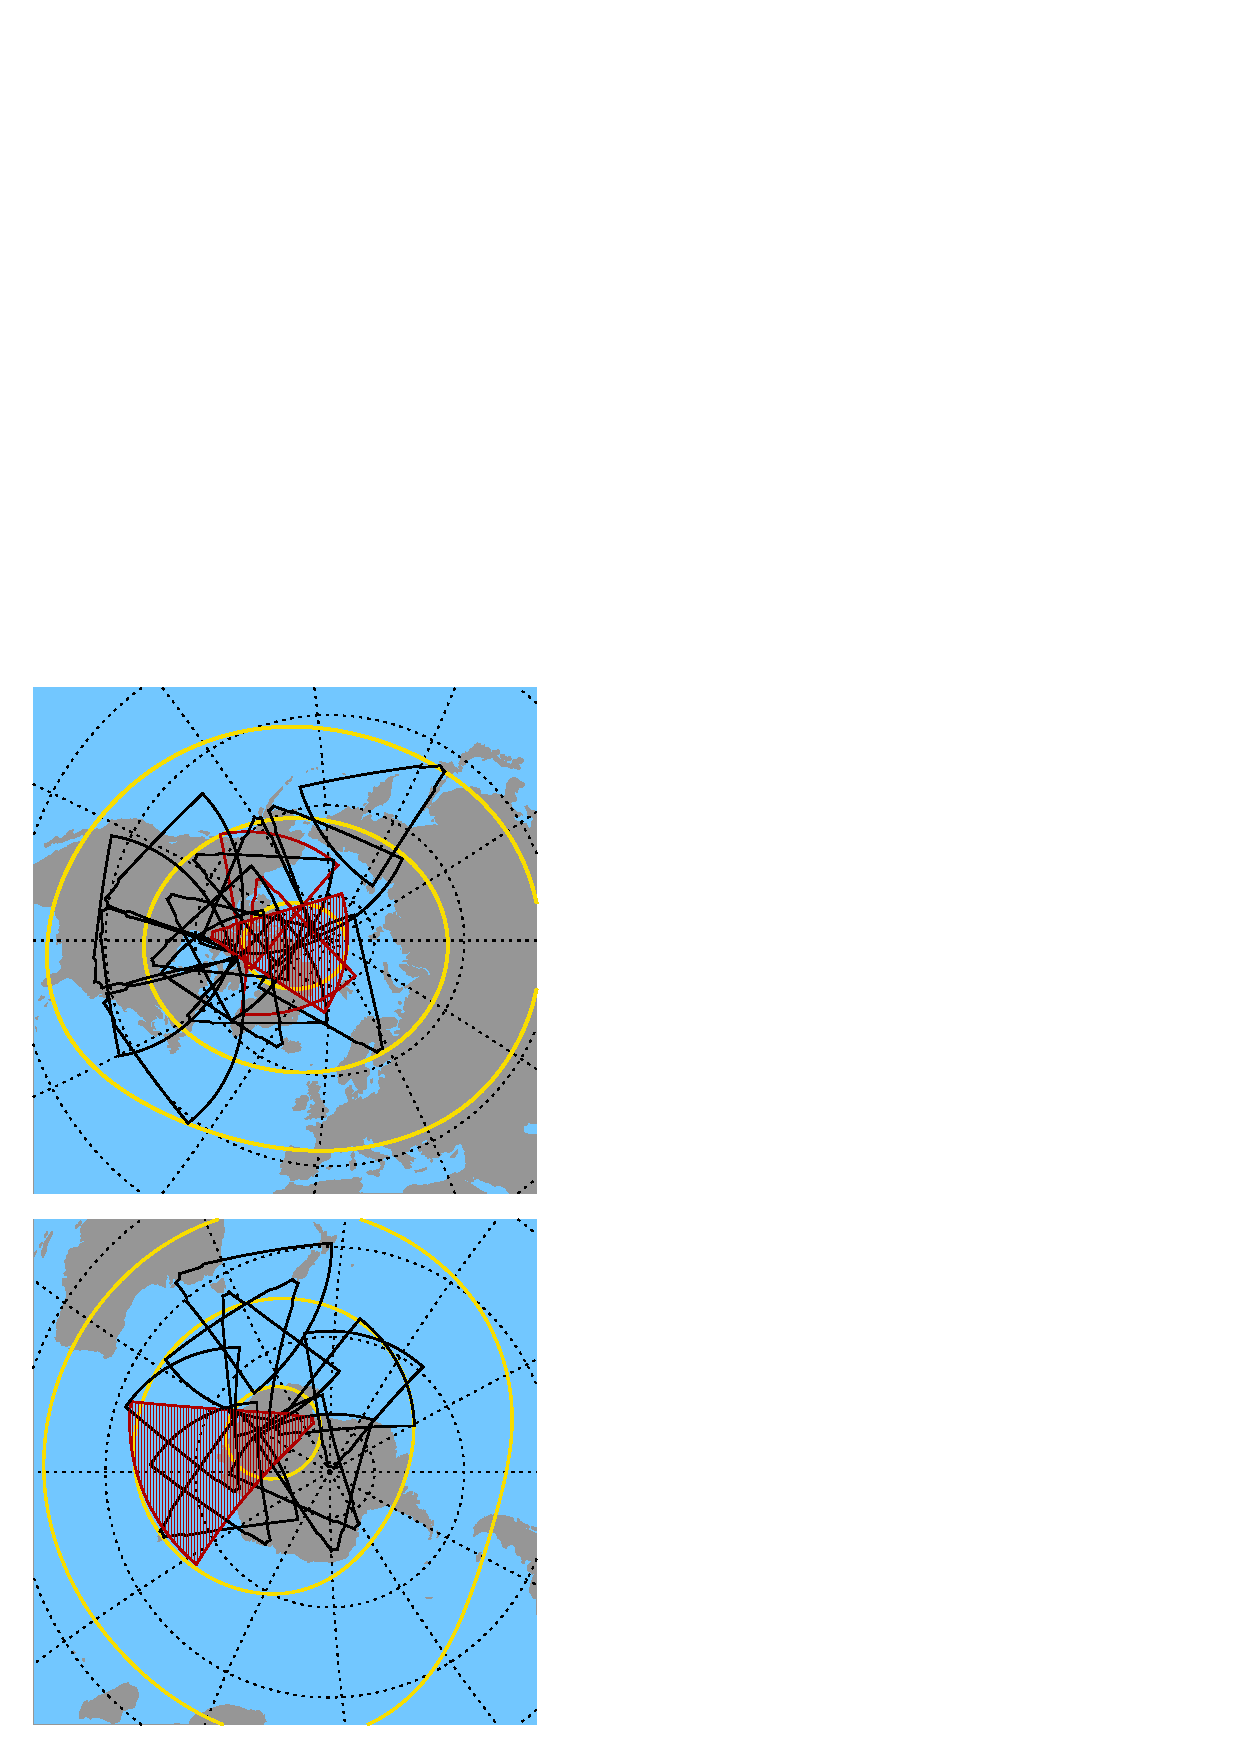
\includegraphics[width=\textwidth,angle=180]{SuperDARNmap.pdf}
	\caption[SuperDARN map]{FoVs of all operational SuperDARN radars in both the northern (left) and southern (right) hemispheres.  Polar latitude radars are shown with the red outlines.  The radars at Rankin Inlet (northern hemisphere) and McMurdo Station (southern hemisphere) are shaded in red because these two instruments are particularly important in the following studies.  Lines of constant magnetic latitude are shown in yellow at \(\Lambda = 40\deg, 60\deg, 80\deg\) in the northern hemisphere and at \(\Lambda = -40\deg,-60\deg,-80\deg\) in the southern hemisphere.}
	\label{fig:superdarnmap}
\end{figure}

It is necessary to use HF radars to study ionospheric structures in the polar cap because the magnetic field is close to vertical and in order for the radar beam to meet the perpendicularity condition to observe FAIs, the beam must be refracted through a dense ionosphere.  VHF radar beams are not refracted enough in the polar cap and the beam will pass through the ionosphere without FAIs producing backscatter.  SuperDARN radars operate nominally between 8--20 MHz, which, according to the Bragg scatter equation for backscatter, corresponds to observing decameter-scale plasma waves.  Each radar consists of 16 independent antennas that transmit a radio wave and receive backscatter from the ionosphere.  Beams are electronically steerable and most radars have between 16 and 24 beams in normal operation mode, each beam being \(3.25\deg\) in azimuth.  Each beam consists of 75--100 range gates, which are generally either 15 km or 45 km in length \citep{Chisham2007}.  SuperDARN radars were originally designed to used a 7 pulse ACF \citep{Farley1972,Greenwald1983,Greenwald1985}, however since 2011, most radars have begun using an 8 pulse sequence.   The multi-pulse increment, \(\tau\), is 2400 \(\mu\)s, which corresponds to a Nyquist frequency of about 200 Hz, small enough to measure plasma drift velocities up to 3000 m/s.  The spectral characteristics of backscatter are derived from the ACF using the FITACF algorithm \citep{Ponomarenko2006}.

One of the original purposes of SuperDARN was to produce maps of the plasma convection patterns in the polar caps using 2D velocity vectors.  Originally this was accomplished by considering two radars with overlapping FoVs.  If both received backscatter from the same scattering volume, two LoS velocities could be found for that scattering volume, which could be combined to find a 2D velocity vector \citep{Ruohoniemi1989}.  The modern method for creating convection maps involves taking all data recorded by all radars in a particular hemisphere and finding the best fit to a 2D ionospheric electrostatic potential using Legendre functions \citep{Ruohoniemi1998}.  For convection maps, only data from the \(F\) region is considered.  If there is not enough velocity data to confine the fit sufficiently, the measured data points are supplemented with a statistical model based on solar wind IMF conditions \citep{Ruohoniemi1995,Ruohoniemi2005}.

Because convection maps require data covering as wide a range of magnetic local time sectors as possible, SuperDARN radars are continuously operational, usually in a common mode.  This creates a vast database of high-quality measurements of small-scale FAIs, which is very useful for other studies on irregularity occurrence and plasma structuring.  In the studies presented here, data was primarily used from the SuperDARN radars located at Rankin Inlet, Canada (RKN) and McMurdo Station, Antarctica (MCM).  These two radars have been shaded in Figure \ref{fig:superdarnmap}.  MCM is the only polar radar in the southern hemisphere.  Although the FoVs of other radars cover parts of the polar cap, they only to at either E region ranges or the furthest of the F region ranges, for which there is rarely much backscatter.  There are currently three polar radars in the northern polar cap, but the FoV of RKN overlaps the Resolute Bay Incoherent Scatter Radar FoV (discussed in Section \ref{sec:isr}, which makes it particularly useful for multi-instrument studies of the ionosphere.

\subsection{Incoherent Scatter Radar}
\label{sec:isr}
Similar to CSRs, incoherent scatter radars (ISRs) are ground based radars that are used to probe the ionosphere.  However, they use a fundamentally different technique to observe structuring, which allows them to measure bulk plasma parameters in contrast to small-scale irregularity characteristics.  While CSRs receive backscatter from relatively large, ``coherent'' density structures in the ionosphere, ISRs operate by radar scattering from waves due to the random thermal motion of electrons in the plasma.  The radar receivers then measure a spectrum of frequencies with different power \citep{Gordon1958}.

The scattering cross section for a volume of N electrons in the ionosphere is given by \(\sigma_n = N \sigma_e\) for radio waves with a wavelength small compared to the Debye length of the plasma, where \(\sigma_e\) is the scattering cross section of a single electron \citep{Gordon1958,Fejer1960}.  The relationship to the plasma Debye length is important because at scale sizes smaller than the Debye length, the plasma is not capable of organized motion, so the motion of the elections is only due to their own thermal energy and not larger scale plasma waves.  The signal returned from this kind of scatter was postulated to have a very low power and a very broad spectral width, however after the first ISR was built, the spectrum was found to be much narrower than previously expected \citep{Evans1969}.  This can be attributed to the effect that the much slower ions have on free electrons in the plasma through ion acoustic waves \citep{Bowles1958}.  The practical results of this is that ISRs can use radio waves of a much longer wavelength than originally anticipated, on the order of \(\sim\)1 m.

Analysis of the returned power spectrum reveals the electron density, electron and ion temperatures, and LoS ion velocity \citep{Evans1969,Rishbeth1985,Nicolls2007a}.  Using a model of chemical composition at different altitudes, the average ion mass can also be found.  In addition, 3D convection velocities and electric field vectors can be derived from LoS ion velocity measurements in some of the more modern ISRs by assuming both \(\vec{E}\) and \(\vec{V}_E\) are constant across the radar's FoV \citep{Heinselman2008}.  More recently, a new algorithm has been developed that used the Lagrange method of undetermined multipliers to generate 3D convection velocity and electric field vectors without making this limiting assumption \citep{Nicolls2014}.  Each instrument must be calibrated with known electron density measurements to account for noise and system constants \citep{Nicolls2007a}.  This is done using the plasma frequency measured from either the plasma line of the ISR spectra during summer daytime period or ionosonde measurements for all other times \citep{Bahcivan2010,Themens2014}.

\begin{figure}
	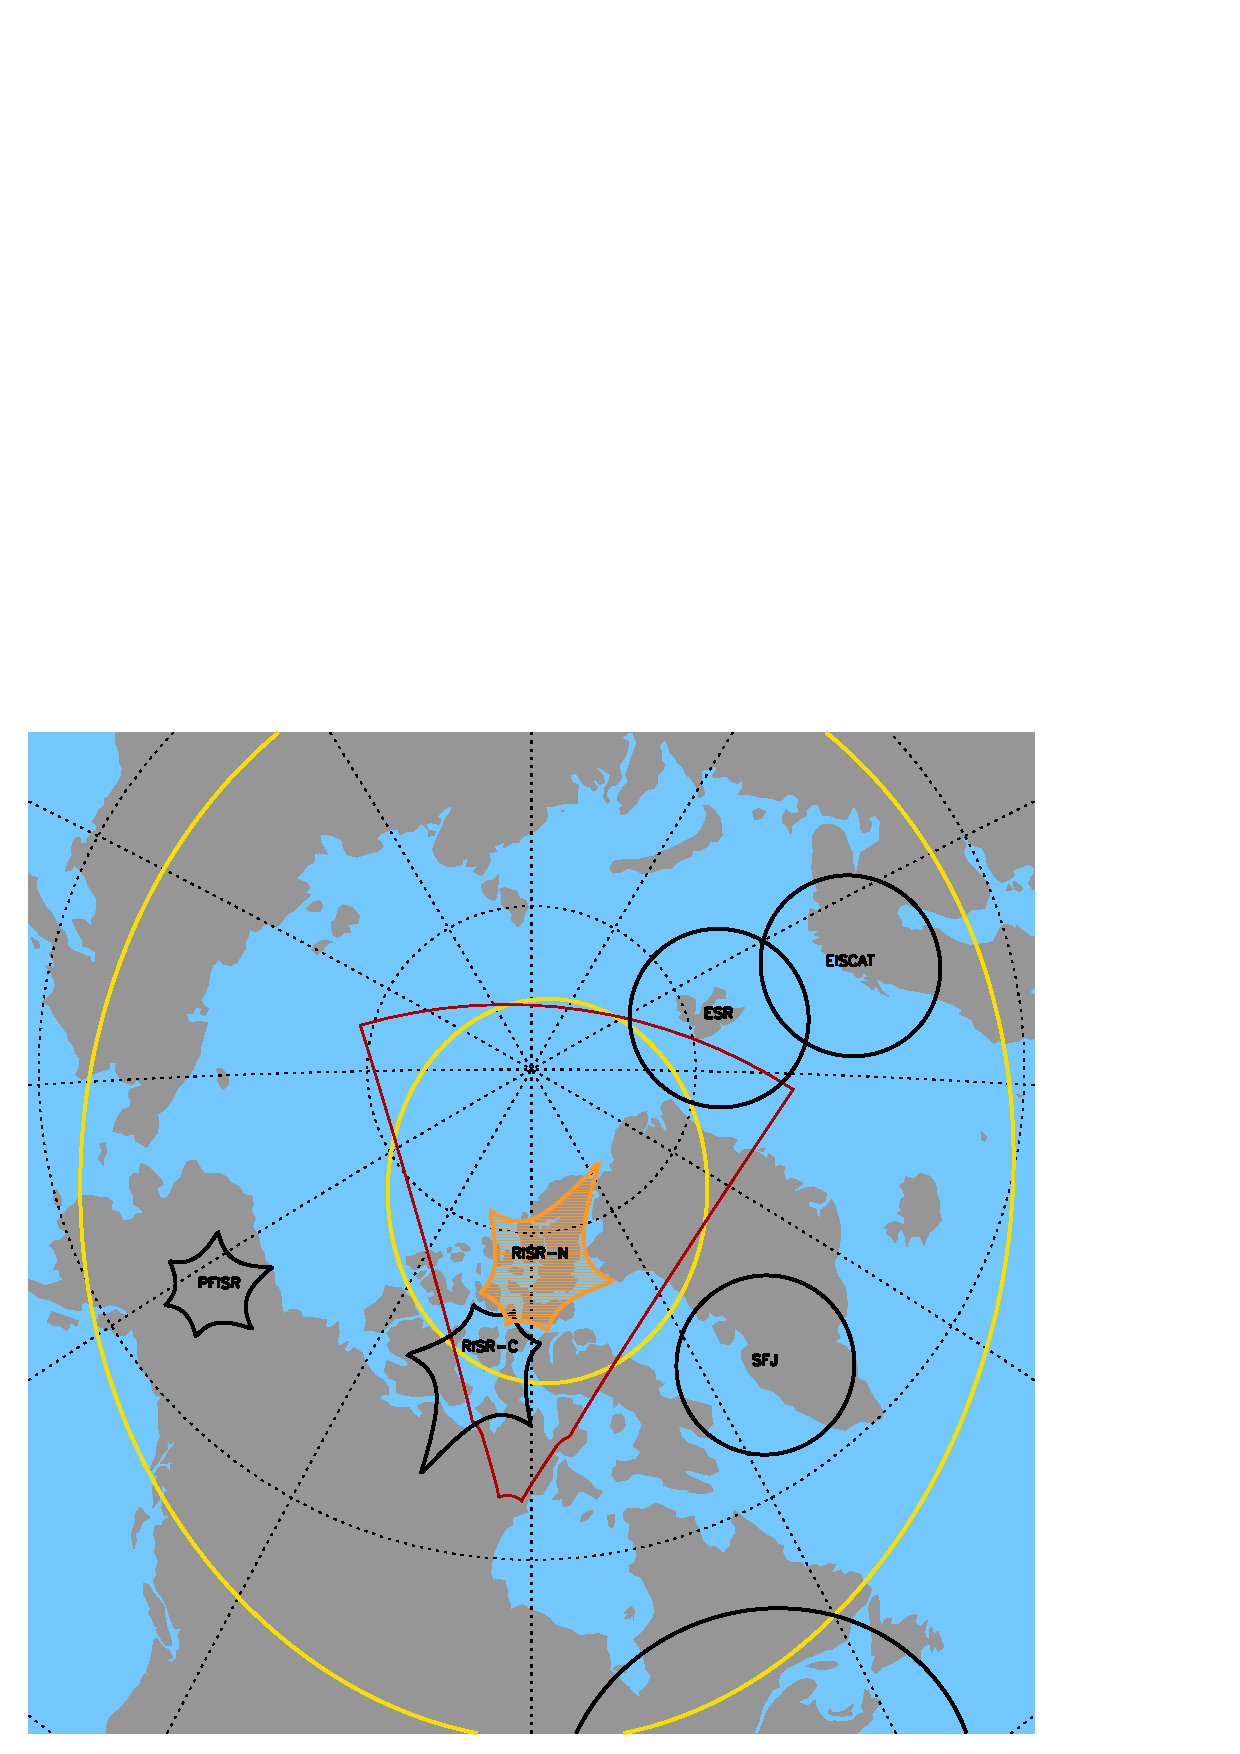
\includegraphics[width=\textwidth]{ISRmap.pdf}
	\caption[ISR map]{FoVs of all ISRs in the northern polar region.  The individual radars shown are identified by their commonly used acronyms: Poker Flat (PFISR), Resolute Bay North (RISR-N), Resolute Bay Canada (RISR-C), Sondrostrom (SFJ).  RISR-N, which is primarially used throughout this thesis, is shown in orange.  The FoV of the RKN SuperDARN radar is shown by the red outline.  Lines of constant MLAT are shown at \(\Lambda=80\deg,60\deg\) in yellow.}
	\label{fig:isrmap}
\end{figure}

The first ISR was built in Arecibo, Puerto Rico in the 1950s \citep{Gordon1958}.  Since then, at least 8 other ISRs have been deployed around the world at equatorial, mid-, and high-latitudes.  A map of the ISR systems currently operational in the northern polar cap is shown in Figure \ref{fig:isrmap}.  The most recent advancement has been the development of Advanced Modular Incoherent Scatter Radars (AMISR), of which there are currently three in use, one at the Poker Flat Rocket Range (PFISR), just north of Fairbanks, Alaska and two in Resolute Bay, Canada (RISR-N and RISR-C).  The advantage of these new systems is that they are electronically steerable, unlike older ISRs which consisted of a large dish that had to be physically moved to change the beam direction.  This allows beams to be transmitted in many different directions at a very high time cadence, giving the radar the capability to make measurements in multiple directions almost simultaneously \citep{Nicolls2007a,Nicolls2007b,Bahcivan2010}.  This is very important for creating 2D maps of ionospheric conditions and tracking how they change in time \citep{Semeter2009,Dahlgren2012a,Dahlgren2012b}.

AMISR systems typically have two types of pulses, a long pulse (LP) with 72 km range gates for \(F\)-region studies and an alternating code pulse (AC) with 4.5 km range gates gates for \(E\)-region studies.  The exact number and configuration of beams depends on the radar mode used and can be changed easily due to the system's electronic steering.  In the common WorldDay mode, there are typically 11 beams and data is collected at \(\sim\)1 min intervals, although this can change slightly between different renditions of the WorldDay mode.  WorldDay mode creates the characteristic star shaped FoV seen in Figure \ref{fig:isrmap}

One of the most important advantages of ISR systems over CSRs is the ability to directly measure electron density in the ionosphere.  However, because ISRs are much scarcer and are only typically run on in WorldDay mode a few days out of every month, data are not as widely available.  In addition, ISRs do not actually observe small-scale coherent plasma structures like the SuperDARN HF network does.  However, they can directly measure large-scale structures and image density variations on scales larger that 100 km (limited by the number of beams and range gate size).  For these region, it is often useful use a combination of CSR and ISR measurements in ionospheric plasma structuring studies, when possible.  The primary ISR used in the present volume of work is the north face of the AMISR system at Resolute Bay, Canada, RISR-N, shown in orange in Figure \ref{fig:isrmap}.  The FoV of RISR-N overlaps that of the RKN SuperDARN radar, red outline in Figure \ref{fig:isrmap}, making it ideal for these types of comparison studies, Chapters \ref{sec:paper1} and \ref{sec:paper3}.

\subsection{IRI Model}
\label{sec:iri}
In addition to radars, models can be a useful tool for understanding the background conditions in the ionosphere, particular in regions where there is poor instrumental coverage.  The International Reference Ionosphere (IRI) is an empirical model of the Earth's ionosphere.  It was originally created in 1969 as a joint effort between the Committee on Space Research (COSPAR) and the International Union of Radio Science (URSI) and has been periodically updated since then \citep{Rawer1975,Rawer1978,Rawer1981,Bilitza1985,Bilitza1986,Bilitza1990,Bilitza1997,Bilitza2001,Bilitza2008}.  The current version is IRI-2012 \citep{Bilitza2014}, which is used throughout the work done here.

The IRI model produces outputs of electron density, temperatures of electrons, ions, and neutrals, ion composition (O\(^+\), H\(^+\), He\(^+\), O\(_2^+\), NO\(^+\), N\(^+\)), and total electron content (TEC).  The model requires the input of a location (latitude, longitude, and altitude) and time (year, date, and time).  Additionally, the model gives the option to choose between two F peak models and three bottomside thickness models.  There are a variety of other optional input parameters such as sunspot number, ionospheric index, and F10.7 radio flux which can help make the output parameters more accurate for a particular situation.  Additionally, the model is capable of producing profiles of any of the output parameters in either space or time.  This is particularly significant for height profiles, and allows the peak heights and densities of the \(E\) and \(F\) region to be calculated.

Although the IRI model is very useful for providing background plasma density conditions where no instruments are available to make measurements, it is important to bear in mind that it is a model and therefor only represents the average conditions.  Although it is fairly accurate at mid-latitudes \citep{Coisson2006,Bilitza2012}, it does not necessarily represent variations within the polar cap well \citep{Themens2014,Makarevich2015b}.  In particular, the height of the F-region peak tends to be underestimated in daytime and the bottomside thickness does not show realistic seasonal and diurnal variation \citep{Themens2014}.  

Despite this, the IRI model is still a very important tool for establishing a density profile at any time in any location in the ionosphere.  And example of an altitude profile of plasma density provided by the IRI model is shown in Figure \ref{fig:densprofile}.  The displayed profiles shows how the electron density changes with altitude at local noon (day) and midnight (night) on January 1, 2007 at \(75\deg\) N, \(0\deg\) E, geographic.

One of the most important uses of the IRI model has been its integration into ray tracing simulations.  Throughout this work, it is valuable to determine the degree to which HF radar beams refract through a dense ionosphere.  This can be done through standard raytracing tools based on numerical solutions to the Hamiltonian raypath equations, as shown in Chapter \ref{sec:paper1} \citep{Haselgrove1963,Jones1975}, however these tools require a 2D density profile along the path that the radar beam travels.  It is possible to assume a Gaussian distribution or Chapman layer as a simple model of the F-region peak, but it is much more instructive to use output from the IRI model, as is done in this work, as it is sensitive to changes in latitude as well as seasonal and diurnal variations.

\section{A Brief Review of Plasma Structuring Theory and Observations in the Polar Cap}
Much work has been done over the past several decades to study the complicated picture of plasma structuring in the polar cap, including theoretical analysis of plasma dispersion relations, simulations of plasma dynamics, and observations of plasma structuring using a variety of instruments.  Here, a survey will be given of some of these advancements and the current state of understanding plasma structuring on a range of scales.

\subsection{Polar Patch Formation}
\label{sec:lit_patches}
Large-scale structuring in the polar cap can take a variety of forms, Section \ref{sec:polar_structure}, but here we will focus on large regions of enhanced plasma density known as polar patches  \citep[e.g.][]{Weber1984,Weber1986,Buchau1983,Buchau1985}.  One of the primary interests of this thesis is the relationships between irregularities of different scales and small-scale structuring has long been observed around polar patches \citep{Weber1984,Milan2002b,Moen2012}.  Although small-scale structures have also been observed around sun-aligned arcs \citep[e.g.][]{Koustov2012}, these structures also tend to be more complicated and often are surrounded by intense shears and electric fields \citep{Safargaleev2000,Aikio2002,Kozlovsky2007}.  Additionally, polar patches occur relatively frequently, providing a good opportunity to study irregularity coupling at different scales \citep{Rodger1996}.  In theory, many of the results presented in this work pertaining to the strong gradients on the edges of patches could also easily be applied to the edges of polar holes, but to date, far less attention has been paid to polar holes in the literature, making it challenging to accurately put observations in context \citep{Makarevich2015}.

The first observations of polar patches were made in the 1960s by \citet{Hill1963}.  They can range in size from 100 km up to 1500 km in diameter and can have peak densities as much as eight times that of the background ionospheric plasma \citep{Weber1986,Hosokawa2014}.  Polar patches are know to emerge on the dayside and then propagate with the background plasma convection across the polar cap to the nightside, where they either disintegrate or recombine with enhanced-density plasma in the auroral oval \citep{Weber1985,Weber1986}.

There have been at least 6 mechanisms proposed for how polar patches form on the dayside \citep{Crowley1996,Carlson2012}:
\begin{enumerate}
	\item Discrete changes in solar wind parameters, usch as IMF, density, speed, and pressure \citep{Sojka1994}
	\item Average flow patterns varying in time \citep{Anderson1988}
	\item Transient magnetopause reconnection \citep{Lockwood1992b}
	\item Plasma production by cusp particle precipitation \citep{Rodger1994,Millward1999}
	\item Plasma flow jet channels that cut continuous streaches of plasma into segments 	\citep{Valladares1998}
	\item Alfven wave coupling \citep{Prikryl1999}
\end{enumerate}.
Although particle precipitation has been shown to create enhanced plasma density in the cusp region \citep{Rodger1994}, it is unreasonable for this mechanism to account for the largest density enhancements observed in polar patches.  These high densities must originate from the reservoir of solar illuminated plasma on the dayside.  Additionally, a mechanism is still required to separate patches from the cusp region.  High speed flow channels can ``cut'' segments off of a tongue of high-density plasma that has been pulled into the polar cap by convection \citep{Valladares1994,Valladares1998}.  Models have also shown that changing large scale convection patterns quickly in time does produce density structures similar to patches \citep{Anderson1988}.  However, the mechanism that seems to be dominant for the majority of polar patches observed is transient magnetic reconnection \citep{Carlson2012}.

In order to discuss patch formation by transient magnetic reconnection, it is important to first understand the steady-state ionospheric convection patterns in the polar cap and how they relate to the magnetosphere \citep{Cowley1980}.  Figure \ref{fig:magnetosphere} is a schematic of how the IMF, magnetosphere, and ionospheric polar cap are all interconnected.  In general, magnetic field lines in the magnetosphere can either be closed (grey lines in Figure \ref{fig:magnetosphere}), meaning they connect only the north and south pole of the Earth, or open (light blue lines in Figure \ref{fig:magnetosphere}), when one of the ends of the field lines originates from the sun such that the field line is connected directly to the IMF.  IMF lines that are not connected to the Earth are shown in dark blue in figure \ref{fig:magnetosphere}.  The polar cap boundary is generally defined as the border between open and closed magnetic field lines, shown by the green line in Figure \ref{fig:magnetosphere}.

By Faraday's Law, the total electromotive force, \(\xi\) around the polar cap boundary is equal to the rate of change of magnetic flux, \(\Phi_B\) within the polar cap, Equation \ref{eqn:pc_imf} \citep{Lockwood1992a}.  In steady-state solutions, \(d\Phi_B/dt = 0\), so \(\xi=0\) by definition, however the polar cap is known to be a highly dynamic system, so changes in magnetic flux are expected.
\begin{equation}
	\label{eqn:pc_imf}
	-\xi = \frac{d\Phi_B}{dt} = B\frac{dA_{pc}}{dt}
\end{equation}
In the polar cap at ionospheric altitudes, the magnetic field strength is relatively constant at around \(5\times 10^-5\) T, so any changes in magnetic flux must be due to changes in the polar cap area, \(A_{pc}\) due to the polar cap boundary expanding or contracting \citep{Lockwood1992a}.  The polar cap boundary changes in response to magnetic reconnection between the magnetosphere and the IMF  on both the day and night sides changing the amount of open magnetic flux.


\begin{figure}
	\includegraphics[width=0.75\textwidth,angle=0]{magnetosphere.pdf}
	\caption[Magnetic reconnection footprint in the ionosphere]{Diagram of the interactions between the IMF, magnetosphere, and polar cap ionosphere.  Closed field lines in the Earth's magnetosphere are shown in grey while open field lines are light blue.  The polar cap open-closed boundary is in green.  Magnetic field lines that are part of the IMF are shown in dark blue.  Magnetic reconnection occurs along the X-line (red) on the dayside of the magnetopause (dashed line).  The X-line can be mapped back along magnetic field lines (orange) to the ionosphere, where their projection is the merging gap (pink dotted line).  During reconnection events, the open-closed boundary expands equatorwards as more open field lines are formed and there is plasma flow across the merging gap. Figure adapted from \citet{Cowley1991}.}
	\label{fig:magnetosphere}
\end{figure}

Magnetic reconnection between the IMF and the Earth's magnetosphere occurs along the X-line on the dayside magnetopause (red line in Figure \ref{fig:magnetosphere}).  The X-line in the magnetopause can be mapped along the magnetic field lines (orange) to the ionosphere, where it is referred to as the merging gap (pink dotted line in figure \ref{fig:magnetosphere}) and lies along the steady state polar cap boundary.  

During reconnection events, the polar cap boundary moves equatorwards as the open magnetic flux into the polar cap increases, Figure \ref{fig:magnetosphere} \citep{Cowley1991,Lockwood1992a}.  In addition, the potential along the X-line also gets mapped to the merging gap, assuming there is minimal drop in potential along the magnetic field lines \citep{Lockwood1992b}.  The combination of these two effects results in flux being transferred across the boundary at a rate equal to the applied voltage  along the X-line and hence plasma flow across the merging gap \citep{Lockwood1992b}, which will be examined further in Figure \ref{fig:patch_formation}.  

Figure \ref{fig:patch_formation} is a schematic of polar patches being formed through transient magnetopause reconnection.  In all panels, the dayside is the top of the figure and the green line shows the open-closed polar cap boundary, similar to Figure \ref{fig:magnetosphere}.  Plasma flow contours are shown in black and the light orange region represents high density from the dayside reservoir.  The reconnection burst starts at Figure \ref{fig:patch_formation}a and the increasing amount of open magnetic flux moves the dayside open-closed boundary equatorwards, as described above \citep{Cowley1991}.

As reconnection continues in Figure \ref{fig:patch_formation}b, the open-closed boundary continues to expand equatorwards as more open flux is produced, which excites a convection pattern in the polar cap \citep{Cowley1991}.  Simultaneously, this convection starts to transport dense dayside plasma polewards \citep{Lockwood1992b}.  As more open flux is produced, Figure \ref{fig:patch_formation}c, the strength of the plasma flow increases and a large blob of dense, dayside plasma is pulled into the polar cap \citep{Lockwood1992b}.

At Figure \ref{fig:patch_formation}d, the burst of reconnection stops and the open-closed boundary begins to relax polewards \citep{Cowley1991}.  As it moves, it pulls the blob of dense plasma within the polar cap with it, separating it from the reservoir on the dayside \citep{Lockwood1992b}.  Before the convection flow stops completely, Figure \ref{fig:patch_formation}e, the blob of dense plasma ``pinches off'' from the dayside plasma to become an independent patch \citep{Lockwood1992b}.  The exact mechanism by which this happens is not well understood, but it is thought to be related to small variations in the IMF By component shifting the convection pattern slightly \citep{Cowley1980,Lockwood1992b}.  By Figure \ref{fig:patch_formation}f, the open-closed boundary has returned completely to its original position and there is a newly formed patch within in the polar cap.  The process can now repeat to form another patch within the polar cap.

A series of reconnection bursts can create a line of patches all propagating across the polar cap.  Reconnection bursts typically last about 2 minutes with anywhere between 7 and 25 minutes between bursts \citep{Foster1984,Etemadi1988,Lockwood1992b}.  However, observations have shown convection flow to be close to continuous for much longer periods.  This can be explained by each reconnection burst exciting flow for a much longer interval than the time between bursts.  In this way, a reconnection burst can excite plasma flow before the convection from the previous burst has stopped, and a series of overlapping reconnection events like this can create continuous plasma flow through the polar cap \citep{Cowley1991}. 

\begin{figure}
	\includegraphics[width=0.75\textwidth,angle=0]{patch_formation.pdf}
	\caption[Polar patch formation]{Polar patch formation through transient magnetopause reconnection.  The open-closed boundary is the green line.  Black contours represent plasma flow.  Dense daytime plasma is shown by the orange regions.  The burst of reconnection is occurring in Figures \ref{fig:patch_formation}a--\ref{fig:patch_formation}c but stops in Figures \ref{fig:patch_formation}d--\ref{fig:patch_formation}f.  Figure adapted from \citet{Cowley1991}.}
	\label{fig:patch_formation}
\end{figure}

\subsection{Theory of Plasma Instabilities}
\label{sec:lit_instabilities}
Plasma structuring, especially at smaller scales, is often discussed in terms of the growth or damping of plasma waves, or instabilities.  As discussed previously in Section \ref{sec:ionosphere_regions}, the plasma characteristics change with altitude in the ionosphere, which causes a variety of different instability mechanisms to be operational depending on the region considered.  The Farley-Buneman instability (FBI), or the modified two-stream instability tends to be a major factor in the \(E\) region where ion inertial effects are strong \citep{Farley1963,Buneman1963}.  Also operational in the \(E\) region but more dominant at higher altitudes is the gradient-drift instability (GDI) \citep{Simon1963,Hoh1963,Linson1970}.  If a wave has a component along the magnetic field line, the current-conductive instability (CCI) can be operational even if GDI is not \citep{Hoh1960,Ossakow1979,Chaturvedi1981}.  Additionally instability mechanisms emerge if shears are considered, when \(\nabla E \neq 0\), such as the Kelvin-Helmholtz instability (KHI) \citep{Kintner1977,DAngelo1965}.

In the polar F-region ionosphere, GDI is typically considered the dominant structuring process \citep{Weber1984,Cerisier1985,Basu1988,Tsunoda1988}.  GDI is operational when high-density perturbations in the plasma move to regions of lower background density and low-density perturbations in the plasma move to regions of higher background density, such that the wave amplitude grows relative to background conditions.  As plasma drifts and carries irregularities with it, electrons and ions have slightly different drifts and create a perturbed electric field.  This perturbed electric field combined with the background magnetic field causes the density perturbations to \(\vec{E}\times\vec{B}\) drift.  If the drift causes high and low density perturbations to move as described above, the instability is operational and the perturbations grow.  If instead high density perturbations drift into regions of higher background density and low density perturbations drift into regions of lower background density, the wave is damped.

Some of the first 1D investigations of the linear GDI growth rate found that it can be described by a simple expression involving the plasma drift speed, \(V_E = |\vec{E}\times\vec{B}|/B^2\), and the gradient scale length, \(L^{-1} = |(\partial n/\partial x)/n|\), Equation \ref{eqn:gdi_old} \citep{Simon1963,Hoh1963,Linson1970}
\begin{equation}
	\label{eqn:gdi_old}
	\gamma = \frac{V_E}{L}
\end{equation}.
This expression is technically only valid if the density gradient, \(\nabla n\), is in the same direction as the plasma drift velocity, \(\vec{V}_E\), and the wave is propagating perpendicular to both.  A more general expression that is used less often, Equation \ref{eqn:gdi_80s}, does consider an arbitrary wavevector, \(\vec{k}\), but still assumes density gradients parallel to the plasma drift \citep{Tsunoda1988}
\begin{equation}
	\label{eqn:gdi_80s}
	\gamma = \frac{k_y}{k}\frac{\vec{k}\cdot\vec{V}_E}{kL}
\end{equation}.
An even more general consideration involves arbitrary gradient and plasma drift directions \citep{Keskinen1982a,Makarevich2014c}.  In this more general case, the directional dependence of GDI has been shown to be significant, such that the growth rate can actually change signs (determining whether wave growth or damping occurs) with different wavevector directions, so it is important to consider this factor \citep{Makarevich2014c}.  In addition, these expressions have historically only applicable in a particular altitudinal regime, usually the F region.

Recently, a new expression has been introduced that considers any arbitrary wavevector, density gradient, and altitude within the ionosphere, which allows three electrostatic instabilities, FBI, GDI, and CCI, to be considered with a single dispersion relation \citep{Makarevich2016a}.
\begin{equation}
	\label{eqn:gdi_Mak16}
	(H_i-H_e)\omega = (H_i\vec{V}_{e0}-H_e\vec{V}_{i0})\cdot\vec{k}+(C_i-C_e)H_eH_i
\end{equation}
As before, \(\vec{k}\) is the wavevector, \(\omega\) is the wave frequency, and \(\vec{V}_{\alpha 0}\) is the background velocity of species \(\alpha\).  The other quantities in equation \ref{eqn:gdi_Mak16} are not standard and described below.
\begin{equation}
	H_\alpha = S_\alpha F_\alpha + D_\alpha^{-1} F_\parallel \quad\quad\quad 
	C_\alpha = \frac{T_\alpha}{m_\alpha \Omega_\alpha}
\end{equation}
\begin{equation}
	F_\alpha = i k_\perp^2 D_\alpha + \vec{G}\cdot\vec{k}_\perp D_\alpha + \vec{G}\cdot\vec{k}\times\uvec{b} \quad\quad\quad
	F_\parallel = i k_\parallel^2 + \vec{G}\cdot\vec{k}_\parallel
\end{equation}
\begin{equation}
	S_\alpha = \frac{1}{1+D_\alpha^2} \quad\quad\quad
	D_\alpha = -\frac{i}{\Omega_\alpha}(\omega-\vec{k}\cdot{V}_{\alpha 0})+r_\alpha
\end{equation}
The quantity \(r_\alpha\) is the ratio of the collision frequency to the gyrofrequency of a particular species, given by \(r_\alpha = \nu_\alpha/\Omega_\alpha\).  

By taking certain limiting cases, expressions for the instability growth rate in different region can be derived from Equation \ref{eqn:gdi_Mak16}.  These expressions are sumarized in Table \ref{tab:gdi_exps}.  In addition to the quantities previously described in relation to Equation \ref{eqn:gdi_Mak16}, the following are useful for the expressions in Table \ref{tab:gdi_exps}.
\begin{equation}
\begin{split}
	b = -\frac{\vec{G}\cdot\vec{k}\times\uvec{b}}{k_\perp^2} \quad\quad\quad
	y = \frac{k_\parallel}{k_\perp} \\
	R = \frac{\sigma_H}{\sigma_P} = \frac{D_i+D_e}{1+\Psi} \quad\quad
	\psi = -r_ir_e \quad\quad
	\hat{\psi} = \psi\left(1+\frac{k_\parallel^2}{r_e^2 k_\perp^2}\right) \\
	\vec{V}_d = \vec{V}_{e0}-\vec{V}_{i0} = (r_i-r_e)\left[s_es_i(1+\psi)\left(R\vec{V}_E-\frac{\vec{E}}{B}\right)\right]
\end{split}
\end{equation}

For the purposes of this thesis, the cold plasma limit expression in Table \ref{tab:gdi_exps} is most recent and can be rewritten using the definition of \(b\), Equation \ref{eqn:gdi} \citep{Makarevich2014c,Makarevich2016a}.
\begin{equation}
	\label{eqn:gdi}
	\gamma = \frac{1}{1+\psi}\left(\uvec{k}\cdot\uvec{b}\times\vec{G}\right)\uvec{k}\cdot\left(\frac{\vec{E}}{B}-R\vec{V}_E\right)
\end{equation}
Equation \ref{eqn:gdi} is applicable throughout the \(E\) and lower \(F\) regions.  

%It is useful to express Equation \ref{eqn:gdi_Mak16} in the following equivalent form by defining additional terms.
%\begin{equation}
%	\label{eqn:gdi_Mak16_alt}
%	\left(D_i-D_e\right)\omega = \vec{V}_d\cdot\vec{k}\left(\frac{Z_2}{Z_1}\right) + \left(D_i\vec{V}_{i0}-D_e\vec{V}_{e0}\right)\cdot\vec{k}+(C_i-C_e)k_{\perp}^2\left(\frac{Z_3}{Z_1}\right)
%\end{equation}
%In the \(F\) region where background plasma motion is dominated by electric fields perpendicular to the magnetic field, the differential plasma velocity, \(\vec{V}_d\), can be described as 
%\begin{equation}
%	\label{eqn:gdi_Mak16_Vd}
%	\vec{V}_d = \vec{V}_{e0}-\vec{V}_{i0} = (r_i-r_e)\left[s_es_i(1+\psi)\left(R\vec{V}_E-\frac{\vec{E}}{B}\right)\right]
%\end{equation}
%where, \(s_\alpha = (1+r_\alpha^2)^{-1}\).  Additionally,
%\begin{equation}
%\label{eqn:gdi_Mak16_Z}
%\begin{split}
%	Z_1 = i(1+Y)+a+Rb+ycK \quad\quad\quad 
%	Z_2 = R(i+a)-b \quad\quad\quad\quad\quad\quad\\
%	Z_3 = -\frac{\Psi(i+a)^2}{1+\Psi}-Rb(i+a)+\frac{b^2}{1+\Psi}-iy(y-ic)\left[\left(K+1-\Psi^{-1}\right)(i+a)+Rb\left(1-\Psi^{-1}\right)\right]\\+Ky^2(y-ic)^2
%\end{split}
%\end{equation}
%and
%\begin{equation}
%\begin{split}
%	a& = \frac{\vec{G}\cdot\vec{k}_\perp}{k_\perp^2} \quad\quad\quad
%	b = -\frac{\vec{G}\cdot\vec{k}\times\uvec{b}}{k_\perp^2} \quad\quad\quad
%	c = \frac{\vec{G}\cdot\vec{k}_\parallel}{k_\perp k_\parallel} \\
%	\Psi = -D_iD_e& \quad\quad
%	R = \frac{D_i+D_e}{1+\Psi} \quad\quad
%	y = \frac{k_\parallel}{k_\perp} \quad\quad
%	K = \left(1+\frac{1}{\Psi}\right)\left(1+R^2\right) \quad\quad
%	Y = Ky^2
%\end{split}
%\end{equation}.

%By considering certain limiting cases, an expression that is more relevant to the polar F region specifically can be resolved from Equation \ref{eqn:gdi_Mak16_alt}.  First, assume a cold plasma such that the temperature of both ions and electrons is negligible.  In this case, \(T_\alpha = 0\), so \(C_\alpha = 0\).  Secondly assume all irregularities are perfectly aligned with the magnetic field such that \(k_\parallel = 0\).  This means that \(\vec{k}_\perp = \vec{k}\), \(y=0\), and \(Y=0\).  Finally, consider only low frequencies (\(\omega \ll \Omega_\alpha\)) and long wavelengths (\(\vec{k}\cdot\vec{V}_{\alpha 0} \gg \nu_\alpha\)).  If \(D_\alpha\) is expressed as shown below, it can bee seen that these limits result in the first two terms being negligible such that \(D_\alpha \approx r_\alpha\).
%\begin{equation}
%	D_\alpha = -i\frac{\omega}{\Omega_\alpha} + i\frac{\vec{k}\cdot\vec{V}_{\alpha 0}}{\Omega_\alpha} + \frac{\nu_\alpha}{\Omega_\alpha} \approx \frac{\nu_\alpha}{\Omega_\alpha} = r_\alpha
%\end{equation}
%Equation \ref{eqn:gdi_Mak16_alt} can then be expressed as follows.
%\begin{equation}
%	\label{eqn:gdi_Mak16_Freg}
%	(r_i-r_e)\omega = \vec{V}_d\cdot\vec{k}\left(\frac{Z_2}{Z_1}\right)+(r_i\vec{V}_{i0}-r_e\vec{V}_{e0})
%\end{equation}
%The growth rate, \(\gamma\), is contained within the dispersion relation as \(\omega = \omega_r+i\gamma\), so the imaginary part of Equation \ref{eqn:gdi_Mak16_Freg} must be considered separately.
%\begin{equation}
%	\label{eqn:gdi_Mak16_gam}
%	(r_i-r_e)\gamma = \vec{V}_d\cdot\vec{k}\;\text{Im}\left\{\frac{Z_2}{Z_1}\right\}
%\end{equation}
%The differential plasma drift has been defined previously in Equation \ref{eqn:gdi_Mak16_Vd} but the imaginary component of \(Z_2/Z_1\) must still be identified.  Using the definitions of \(Z_1\) and \(Z_2\) provided in Equation \ref{eqn:gdi_Mak16_Z} and the simplifying assumptions discussed above for the F region,
%\begin{equation}
%	\frac{Z_2}{Z_1} = \frac{R(i+a)-b}{i+a+Rb}
%\end{equation}.
%Multiplying both the numerator and denominator by \(-i+a+Rb\) removes the imaginary component from the denominator.  Additionally the local approximation \(G \ll k_\perp\) is taken, which results in \(a\), \(b\), and \(c\) being small so that any second order terms in these quantities can be neglected.
%\begin{equation}
%	\frac{Z_2}{Z_1} = R+ib(1+R^2)
%\end{equation}
%Using the above result and Equation \ref{eqn:gdi_Mak16_Vd}, Equation \ref{eqn:gdi_Mak16_gam} becomes
%\begin{equation}
%	(r_i-r_e)\gamma = (r_i-r_e)s_es_i\left(1+\psi\right)\left(R\vec{V}_E-\frac{E}{B}\right)\cdot\vec{k}b\left(1+R^2\right)
%\end{equation}
%Recognizing that \(s_es_i\left(1+R^2\right) = (1+\psi)^{-2}\) and \(b = \vec{G}\cdot\vec{k}\times\uvec{b}/k^2 = -\vec{k}\cdot\uvec{b}\times\vec{G}/k^2\) by vector identities, a final expression for the GDI growth rate in the F region can be found, which agrees well with the results of \citet{Makarevich2014c}
%\begin{equation}
%	\label{eqn:gdi}
%	\gamma = \frac{1}{1+\psi}\left(\uvec{k}\cdot\uvec{b}\times\vec{G}\right)\uvec{k}\cdot\left(\frac{\vec{E}}{B}-R\vec{V}_E\right)
%\end{equation}.
%Equation \ref{eqn:gdi} will be critical to the analysis done both in Chapter \ref{sec:paper2} and Chapter \ref{sec:paper3} in this thesis.

\begin{table}
\begin{tabular}{l l}
Limiting Case & Growth Rate, \(\gamma\) \\
\hline
GDI/FBI in \(E\) Region & \(\gamma = \frac{1}{1+\hat{\psi}}\left[\frac{\hat{\psi}}{\nu_i}\left(\left(\frac{\vec{V}_d\cdot \vec{k}}{1+\hat{\psi}}\right)^2-C_s^2 k_\perp^2\right)+\frac{br_i\vec{V}_d\cdot \vec{k}}{1+\hat{\psi}}\right]\) \\
GDI/CCI in \(F\) Region & \(\gamma = -\frac{b}{\psi+y^2}\left[\frac{\psi\vec{k}\cdot\vec{E}_{0\perp}+E_{0\parallel}k_\parallel}{B}\right]+C\left[r_ek_\perp^2-\frac{k_\parallel^2}{r_i}\left(1+\frac{r_i^2}{\psi+y^2}\right)\right]\) \\
Cold Plasma in \(F\) Region & \(\gamma = \frac{b}{1+\psi}\left(R\vec{V}_E-\frac{\vec{E}_{0\perp}}{B}\right)\cdot\vec{k}\) \\
\end{tabular}
\caption[Irregularity growth rates]{Irregularity growth rates in the ionosphere for three different limiting cases \citep{Makarevich2016a}.}
\label{tab:gdi_exps}
\end{table}

Although linear GDI theory as described predicts clear dependence on wave vector direction \citep{Makarevich2014c}, this theory is only really valid in the long-wavelength limit, \(\vec{k}\cdot\vec{V}_E \ll \nu_\alpha\).  In the \(F\) region, the ion-neutral collision frequency, \(\nu_i\), is about 10 Hz and if the drift speed, \(V_E\), is about 1000 m/s, fluid theory only applies for wavelengths greater than 100 m, larger than the decameter-scale waves that are detected by SuperDARN.  This raises the important question of whether or not the same anisotropy that is predicted by linear GDI theory at larger scales can be expected in small-scale irregularities where nonlinear processes may be important.  This issue has mostly been studied through numerical simulations due to the challenges associated with measuring a high-resolution 2D spectrum experimentally.

The first simulations of GDI were done in the 1970s and successfully reproduced structures developing on the trailing edge of large density gradients \citep{Zabusky1973,Doles1976,Scannapieco1976,Ossakow1975,Ossakow1977}.  Later, 2D simulations were expanded to include magnetosphere-ionosphere coupling, but it was found that this only had a substantial effect for very large-scale structures \citep{Keskinen1990}.  3D simulations were introduced of GDI surrounding a large plasma density enhancement \citep{Guzdar1998} and were later improved by including plasma dynamics parallel to the magnetic field and inertial effects so that secondary KHI and tertiary shear-driven instability processes could be modeled \citep{Gondarenko1999}.  These simulations consistently showed asymmetry between the leading and trailing edge of large-scale density structures and fluctuations in plasma density that were as much as 10--20\% of the background plasma \citep{Gondarenko2004a,Gondarenko2004b}.  Plasma structuring can occur on the leading edge of large-scale density enhancements if the convection velocity changed rapidly such that the trailing edge becomes the leading edge and vice versa, or if there are large velocity shears initially present \citep{Gondarenko2004a,Gondarenko2004b}.

For the most part, the results of nonlinear numerical simulations very closely match expectations from linear GDI theory.  The spatial power spectra are anisotropic with most of the power concentrated in the direction where linear GDI growth is most favorable \citep{Keskinen1981a,Keskinen1981b,Keskinen1982a,Gondarenko2001,Gondarenko2004b}.  However, very strong shears or increasing the impact of ion-inertial factors can cause isotropy \citep{Gondarenko2001,Gondarenko2006}.  The power spectra derived from these simulations are similar to those from experimental observations \citep{Baker1978,Kelley1979}, however it is computationally challenging to run simulations down to decameter scales and observations are generally limited to rocket and satellite techniques, which can only be used to calculate power spectra in one dimension \citep{Villain1986,Moen2012}.

%/  Additionally, 2D power spectrum could be calculated and initially considered plasma waves along a large density structure but were later expanded to include magnetosphere-ionosphere coupling \citep{Keskinen1981,Keskinen1982,Keskinen1990}.  

%\citet{Keskinen1982} found plasma waves on the trailing edge of at large density enhancement are unstable.  \citet{Keskinen1990} expanded these results by considering coupling between the magnetosphere and ionosphere, but found that this coupling only has a substantial effect for very large-scale structuring.  In addition, this simulation predicted instability evolution that was far faster than what observations had shown.  3D simulations of GDI surrounding a plasma density enhancement were introduced in \citet{Guzdar1998}.  \citet{Gondarenko1999} improved this 3D simulation further by including plasma dynamics parallel to the magnetic field and inertial effects.  These factors are necessary for the simulation to model secondary KHI and tertiary shear-driven instability processes.  These simulations provided insight in how exactly GDI structuring develops.  

%Both the density and velocity spectra were found to be anisotropic, however increasing the impact of ion-inertial factors in simulations caused both spectra to become more isotropic \citep{Gondarenko2001}.  

%Fluctuations in density were found that were as much at 10--20\% of the background plasma density \citep{Gondarenko2004a}.  Although asymmetry between structuring on the leading and trailing edges of a large-scale density structure was observed in all simulations, rapidly changing convection velocity could complicate this \citep{Gondarenko2004b}.  For instance, if a large scale structure was drifting one direction and convection patters change suddenly so that it is now drifting in the opposite direction, the leading edge becomes the trailing edge and vice versa and both edges may exhibit some structuring.  Additionally, both edges may become structured if large velocity shears are initially present surrounding the density structure \citep{Gondarenko2006}.  Large shears additionally cause KHI to be operational as a primary structuring mechanism, but over time GDI will still be the dominant structuring process.


\subsection{Observations of Polar Cap Structuring}
\label{sec:lit_observations}
Polar patches were first observed in the 1960s \citep{Hill1963}, but much of the work of characterizing them using optical and radio techniques was not accomplished until two decades later \citep{Weber1981,Weber1984,Weber1986,Buchau1983,Buchau1985}.  Polar patches are density enhancements of as much as \(10^6\) cm\(^{-3}\) that occur primarily in the polar \(F\) region \citep{Buchau1983}.  There were initially categorized as extending 800--1000 km horizontally \citep{Weber1984}, but more recent studies have identified patches as large as 1500 km \citep{Hosokawa2014}.  Patches tend to drift antisunwards at speeds of 500--1000 m/s, following background convection \citep{Buchau1983,Weber1984}.

%\citet{Coley1998} examined the occurrence of polar patches in both the northern and southern hemispheres with DE-2 and found that 

Polar patch occurrence varies both diurnally and seasonally, with a diurnal peak at magnetic noon and a seasonal peak during equinox months \citep{Rodger1996}.  Additionally, there is a bias towards patches occurring when there is a negative IMF \(B_z\) component \citep{Buchau1983,Rodger1996}.  The frequency of patch occurrence is greatest when the cusp is slightly daywards of the terminator.  This creates the situation of a dark polar cap, so background plasma density is low and blobs of enhanced density are easily visible \citep{Coley1998}.  In addition, the cusp then provides a gateway of highly ionized sunlit plasma into the dark polar cap.  Patches convect from the dayside through the cusp/throat region towards the polar cap \citep{Kelly1984,Foster1984,Foster1985,Foster1993,Sojka1982,delaBeaujardiere1985}. 

%Several studies had previously reported density enhanced patches convecting from the dayside through the cusp/throat region toward the polar cap \citep{Kelly1984,Foster1984,Foster1985,Foster1993}.  This also agrees with observations made by \citet{Sojka1982,delaBeaujardiere1985}  

%\citet{Rodger1996} also considered occurrence of patches but with a HF radar in Halley, Antarctica.  The diurnal variation in patch occurrence was found to peak at magnetic noon and the seasonal variation in equinox months.  The only correlation between hourly averaged solar wind parameters that was found was a bias towards patches occurring with a negative IMF \(B_z\) component.  

Over time, the trailing edge of a patch became steeper than the leading edge and irregularities developed on the trailing edge.

\citet{Weber1981} identified sun-aligned arcs that extend  along the sun-earth line through large parts of the polar cap using all-sky imaging photometers (ASIP).  These arcs are over 1000 km long and \(\sim100\) km wide and are produced by soft electron precipitation.  

Additionally, \citet{Buchau1983} found that polar patches were more likely to be observed for southward IMF \(B_z\) while sun-aligned arcs were more common for northwards \(B_z\).  

%\citet{Buchau1983} used a combinations of Digisonde and ASIP measurements to identify large luminous patches in the polar cap in addition to sun-aligned arcs.  These patches could have densities up to \(10^6\) cm\(^{-3}\) and tended to drift antisunward.  

%\citet{Weber1984} found patches of enhanced ionization between 800--1000 km during moderately disturbed geomagnetic conditions, again using a combination of ASIP images, ionosonde measurements, and data from Dynamic Explorer 2 (DE-2).  These findings confirmed that density enhancements tended to drift antisunward at speeds of 500-1000 m/s and patches were not colocated with enhanced particle within the polar cap, indicating that this is not the source of the density enhancement.  Over time, the trailing edge of a patch became steeper than the leading edge and irregularities developed on the trailing edge.  

Patches are not colocated with enhanced particle precipitation within the polar cap, indicating that this is not the source of the density enhancement \citep{Weber1984}.  Conversely, \citet{Buchau1985} found that plasma densities within patches were comparable with those measured at dayside sub-auroral latitudes, suggesting that dayside solar-illuminated plasma is the source of dense plasma that form polar patches.

The theoretical mechanism for patch formation via transient magnetic reconnection has been described previously, Section \ref{sec:patch_formation}.  A variety of experimental evidence has been presented to support this mechanism \citep{Cowley1998,Carlson2002}.  Experiments run in the 1980s using the European Incoherent Scatter Scientific Association (EISCAT) Troms\o, Norway ISR showed that plasma flow occurred near noon shortly after southward IMF \(B_z\) arrives at the magnetopause \citep{Etemadi1988,Todd1988}.  These plasma flows are pulsed in the region of the polar cap boundary \citep{Lockwood1993a,Lockwood1993b}, as predicted by \citet{Cowley1991}.  Observations made by an ASIP in Svalbard in 1984 are fully consistent with patch formation through transient magnetopause reconnection \citep{Carlson1996,Carlson2002}.  \citet{Carlson2004} identified five signatures of transient magnetic reconnection and then examined a patch formation event for these signatures using the EISCAT Svalbard Radar.  All five signatures were observed as expected, strengthening the idea that transient magnetopause reconnection is responsible for patch formation.  Furthermore, \citet{Carlson2006} identified and tracked a series of patches directly from the subauroral plasma reservoir and show that the boundary moves equatorwards before relaxing poleward, one of the main predictions of the transient magnetopause reconnection mechanism \citep{Lockwood1992b}.  A review of historical observations of polar patches has been provided by \citet{Crowley1996}.



Recent advancements have improved the ability to image density structures in the ionosphere, particularly using multi-instrument approaches.  \citet{Semeter2009} introduced a method by which the density pattern in a particular volume could be imaged in three dimensions using AMISR systems.  This technique was later used by \citet{Dahlgren2012a,Dahlgren2012b} to image a polar patch.  \citet{Dahlgren2012b} additionally used ASIPs and SuperDARN radars to investigate the polar patch and found that backscatter tended to be observed more on the trailing edge of the patch.  This agrees well with many studies that have examined the asymmetry of small-scale plasma structuring surrounding plasma patches.  

Over time, the trailing edge of a patch became steeper than the leading edge and irregularities developed on the trailing edge \citep{Weber1984}.  Backscatter power from HF radars tends to be greater on the trailing edges of both moving high-density polar structures \citep{Milan2002b} and sun-aligned arcs identified from ASIP data \citep{Koustov2012}, which is generally attributed to GDI being unstable on the trailing edge but stable on the leading edge of such large, moving density structures.  Studies of patches using all-sky airglow imagers (ASI) found that the density gradient on the leading edge of polar patches tends to be 2--3 times steeper than that on the trailing edge \citep{Hosokawa2016}.  Additionally, large finger-like structures on the trailing edge of patches have been identified that were 10s--100s of kilometers in size and agree with predictions made by GDI simulations \citep{Gondarenko2004b}.  \citet{Moen2012} made direct measurements of plasma density structuring using the ICI-2 sounding rocket.  This study provided evidence that decameter scale plasma structuring (the same as observed by HF radars) had spawned from kilometer scale density gradients (that observed by ASIP and ASI methods) and structuring was greatest where GDI was operational.

Small-scale plasma irregularities are typically studied with HF coherent scatter radars in the polar cap, Section \ref{sec:csr}.  The factors that affect irregularity observation can roughly be divided into two groups, irregularity production and radar propagation.  Irregularity production factors are related to the existence of plasma irregularities in the ionosphere while radar propagation factors are related to the ability to observe irregularities with a ground based radar, Section \ref{sec:superdarn}.  Within the polar caps, plasma irregularity production is much higher than at lower altitudes such that when background plasma conditions are favorable for radar propagation, FAIs are observed nearly continuously \citep{Bristow2011}.  However, there are still definite diurnal, seasonal, and solar cycle trends \citep{Kane2012}.  There is an increase in echo occurrence at solar maximum, particularly in the midnight sector \citep{Milan1997,Koustov2004}.  Seasonally, high latitude radars observe a peak in echo occurrence during equinox months \citep{Koustov2004}.  Additionally, backscatter tends to occur at closer ranges in summer at midnight, but moves further away from the radar in other seasons at midday \citep{Milan1997}.  In general, echo occurrence in high during the day and low at night, but nighttime occurrence is directly proportional to the \(F\) peak density and daytime occurrence can be significantly reduced by a dense and conductive \(E\) layer. \citep{Koustov2004,Kane2012,Vickrey1982}.  In the daytime, solar illumination causes the electron density of the \(E\) region to increase dramatically, making it highly conductive.  This conductive layer can provide a conduit by which the potential differences associated with FAIs in the \(F\) region can be shorted out, effectively reducing \(F\)-region plasma irregularities \citep{Vickrey1982}.  Both irregularity production and radar propagation factors probably contribute to these regular variations of echo occurrence, because while a dense, daytime ionosphere creates favorable radar propagation conditions, it can also contribute to \(E\)-region shorting or smoothing of gradients which surpress irregularity production \citep{Koustov2004}.  

Irregularity production is impacted primarily by the presence of strong density gradients and electric fields in the ionosphere \citep{Koustov2004}.  Properly oriented density gradients and electric fields are a necessary condition for GDI to be operational, Section \ref{sec:lit_instbilities}, so the stronger these are, the more likely the irregularity production rate is high.  Both backscatter power and occurrence increase with increasing electric field strength \citep{Ballatore2001,Danskin2002,Makarevich2014b}.  Similarly, backscatter occurrence increases when the IMF \(B_z\) component is strongly negative, implying a strong merging electric field.

The primary radar propagation factor to consider is the background plasma density and how much the radar beam is refracted.  If the background density is too low, the beam is under refracted and is never perpendicular to the magnetic field, however if the density is too high, the beam is over refracted, such that observation of small-scale FAIs is most favorable if the background density is between \(1\times 10^{11}\) m\(^{-3}\) and \(4\times 10^{11}\) m\(^{-3}\) \citep{Danskin2002,Makarevich2014b}.  If the \(D\) region is too dense, this can also in theory attenuate the signal and reduce the rate of returned backscatter, although observations have shown this is not a major factor in echo occurrence \citep{Danskin2002}.  Finally, the radar equation predicts that the returned backscatter should be proportional to the perturbation density, \(\delta n\), squared, or, equivalently, the product of the background density and the fractional density, \(\delta n/n\), squared, Equation \ref{eqn:fractional_density}
\begin{equation}
	\label{eqn:fractional_density}
	P \propto \delta n^2 \propto \left(\frac{\delta n}{n}\right)^2 n^2
\end{equation}.
There is no general agreement of what controls the fractional density, however, if it is approximately constant, then radar backscatter power could be directly proportional to \(n^2\).


\section{Motivation and Objectives}

The plasma in the polar cap ionosphere is highly structured in a non-trivial manner \citep{Tsunoda1988,Carlson2012}.  In addition to being of purely scientific interest, this structuring creates complications when receiving radio signals through the ionosphere.  Because the structuring is highly irregular and varies on many spatial and temporal scales, unpredictable wave refraction, phase shifts, and amplitude attenuation can occur, making signals difficult to detect.  This introduces problems in any system that involves ground-to-satellite, satellite-to-ground, or over-the-horizon communication, such as navigation or communication.  Because of the increasing interconnectedness of modern society, any interruptions or errors in these systems can have broad impacts on infrastructure, including commercial and defense interests, as well as everyday life.

The ionosphere is an important part of the highly coupled Sun-Earth environment.  The polar cap ionosphere essentially serves as the boundary conditions for waves propagating through the magnetosphere.  In addition, understanding plasma structuring on a range of scales is important for correctly interpreting backscatter from ionospheric radars.  In particular, one of the main purposes of SuperDARN is to create large scale convection maps of both polar caps.  These convection maps have been used to give context of both magnetosphere and thermosphere behavior and are widely used in space physics research.  To map convection accurately, it is extremely important to understand when backscatter is observed and when it is absent, and why this is so.  Understanding plasma instability and wave growth mechanisms is very important for answering these kinds of questions.  Models and simulations of structuring in the polar caps incorporate structuring mechanisms so it is helpful if these are better understood, both the operation of a particular mechanism as well as how different mechanism are interconnected and which ones may be dominant under particular conditions.

The aim of this work is to investigate small-scale plasma irregularity production in the \(F\)-region polar cap.  In particular, factors such as direct and indirect global solar control and GDI directional dependance will be considered.  The majority of observational data has been found from ground based ionospheric radars, both CSR systems (Section \ref{sec:csr}) and ISR systems (Section \ref{sec:isr}), with particular emphasis on radars within the SuperDARN network, Section \ref{sec:superdarn}.  However, these datasets have also been supplemented with information from models as well as satellite data when necessary.  Results are investigated in the context of a linear fluid theory analysis of ionospheric plasma.

The first objective of is to evaluate the extent of solar control over irregularity production in the polar \(F\) region.  The occurrence of radar backscatter will be compared with both solar illumination (considered direct solar control) and IMF factors (considered indirect solar control).  This gives a macrophysical view of where and when plasma irregularities are most likely to occur.

The second objective is to investigate asymmetry in the GDI growth rate surrounding large-scale density structures.  A model is used to identifying where plasma irregularities occur surrounding a polar patch and how they can be observed by a ground-based HF radar.  The model considers a large, elongated polar patch drifting in an arbitrary direction relative to a radar and assumes irregularity production is directly dependent to the linear GDI growth rate.  High linear growth rates predicted by the model are compared with classic observations of stronger backscatter power trailing drifting polar patches.

The third objective is to investigate directional dependancies of small-scale plasma irregularities.  Two dimensional measurements of density gradients and electric fields are made such that the directionally dependent GDI growth rate can be calculated, which is then compared with plasma irregularity power and occurrence in a particular location.  This gives insight into whether the production of small-scale irregularities is directionally dependent, similar to the linear GDI growth rate, or if the distribution is isotropic due to other nonlinear processes.

The outline of this thesis is as follows.  Chapter \ref{sec:introduction} has provided an overview of the polar ionosphere and both macro- and microphysical plasma structuring mechanisms.  Chapter \ref{sec:paper1} presents an experimental investigation of decameter-scale plasma irregularities in the polar F-region and their solar control, with a particular focus on statistical analysis of data collected with a recently-deployed SuperDARN radar in the southern polar cap.  The same results were also presented in a recent journal article \citep{Lamarche2015}.  Chapter \ref{sec:paper2} presents a modeling study of the linear GDI growth rate surrounding a large, elongated polar patch drifting in an arbitrary direction within the FoV of a SuperDARN radar uses the results to provide insight as to optimal conditions from radars to observe irregularities.  These results have also been recently published \citep{Lamarche2016}.  Chapter \ref{sec:paper3} presents an experimental investigation of the directional dependence of small-scale plasma structures by considering simultaneous measurements of electric field and density gradients from an AMISR  system and FAIs observed by SuperDARN.  Particular emphasis is placed on if small-scale structures are directionally dependent similar to the predictions of linear GDI theory.  The same results have been submitted for publication \citep{Lamarche2017}.  Chapter \ref{sec:conclusion} presents a summary of the most significant results of this body of work, their implications for interpretation of radar observations of plasma structures in the polar cap and suggestions for future research involving coherent and incoherent scatter radar facilities in the polar region.

\bibliographystyle{uafthesis}
\bibliography{references}

